\documentclass[border=3mm]{standalone}
\usepackage{tikz}
\usetikzlibrary{circuits.ee.IEC}

\begin{document}
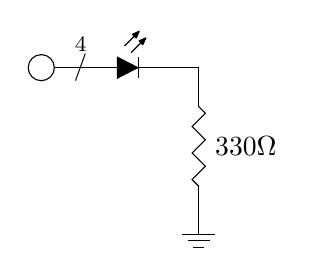
\begin{tikzpicture}[circuit ee IEC,small circuit symbols]
    \node at (0.5,0) {/};
    \node[font=\footnotesize] at (0.5,0.30) {4};
    \begin{scope}[set resistor graphic=var resistor IEC graphic,
                  set diode graphic=var diode IEC graphic]
        \draw (0,0) to[circuit handle symbol={draw,shape=circle,at start}] (0.2,0) to[diode={light emitting}] (2,0) to[resistor={ohm=330},point down] (2,2) to[ground={pos=1}] (2,-2.2);
    \end{scope}
\end{tikzpicture}

\end{document}

